% vim: set tabstop=4 foldmethod=marker foldlevel=0 :
%**********************************************************
%\chapter{一般的にはサーベイ内容とかを書く}
\chapter{人流シミュレーションの高速化}
\label{sec:survey}
%**********************************************************
SFMを用いた人流シミュレーションは,解析人数が多くなるほど計算負荷が
膨大になるため,解析に時間がかかる.
SFMの解析時間を削減するために,モデルの単純化(参考文献)や
エージェント間距離の計算回数削減手法(参考文献),
単位時間あたりの計算回数の増加手法 (参考文献),
経路選択時の判定回数の削減手法(参考文献)などが提案されている.
本章では,SFMの各高速化手法について述べる.

\section{モデルの簡易化}
SFMの簡易化手法は,SFMの計算負荷を削減するために,
エージェント同士や壁や机などの障害物から受ける力,
進行方向を単純化する手法である.
SFMの簡易化手法の一つに一次元歩行者モデルがある(参考文献).
一次元歩行者モデルは,エージェントの動きをxやyのみにする手法である.
図\ref{fig:ichijigen_ex}に避難シミュレーション時のSFMと一次元歩行者モデルの例を示す.
図\ref{fig:ichijigen_ex}中の(a)はSFMなどの二次元連続空間モデルを示し,
(b)は一次元連続歩行者モデルの例を示す.
一次元歩行者モデルは,図\ref{fig:ichijigen_ex}のように,エージェントの動きを
算出する式を一次元に変更することで,計算負荷を削減できる.
本手法は,人の流れ(流量)を解析する場合では,
高速かつ許容できる誤差の範囲で解析できることが報告されている(参考文献).
一方で,一次元でエージェントの動きを再現するため,人の押し合いや
図\ref{fig:atigenshou}のようなアーチ現象などを再現できない.
このため,人の押し合いやアーチ現象を再現したい場合には,
一次元歩行者モデルなどのモデルを簡易化しない高速化技法を用いることが
望ましい.

\begin{figure}[hbtp]
 \begin{center}
  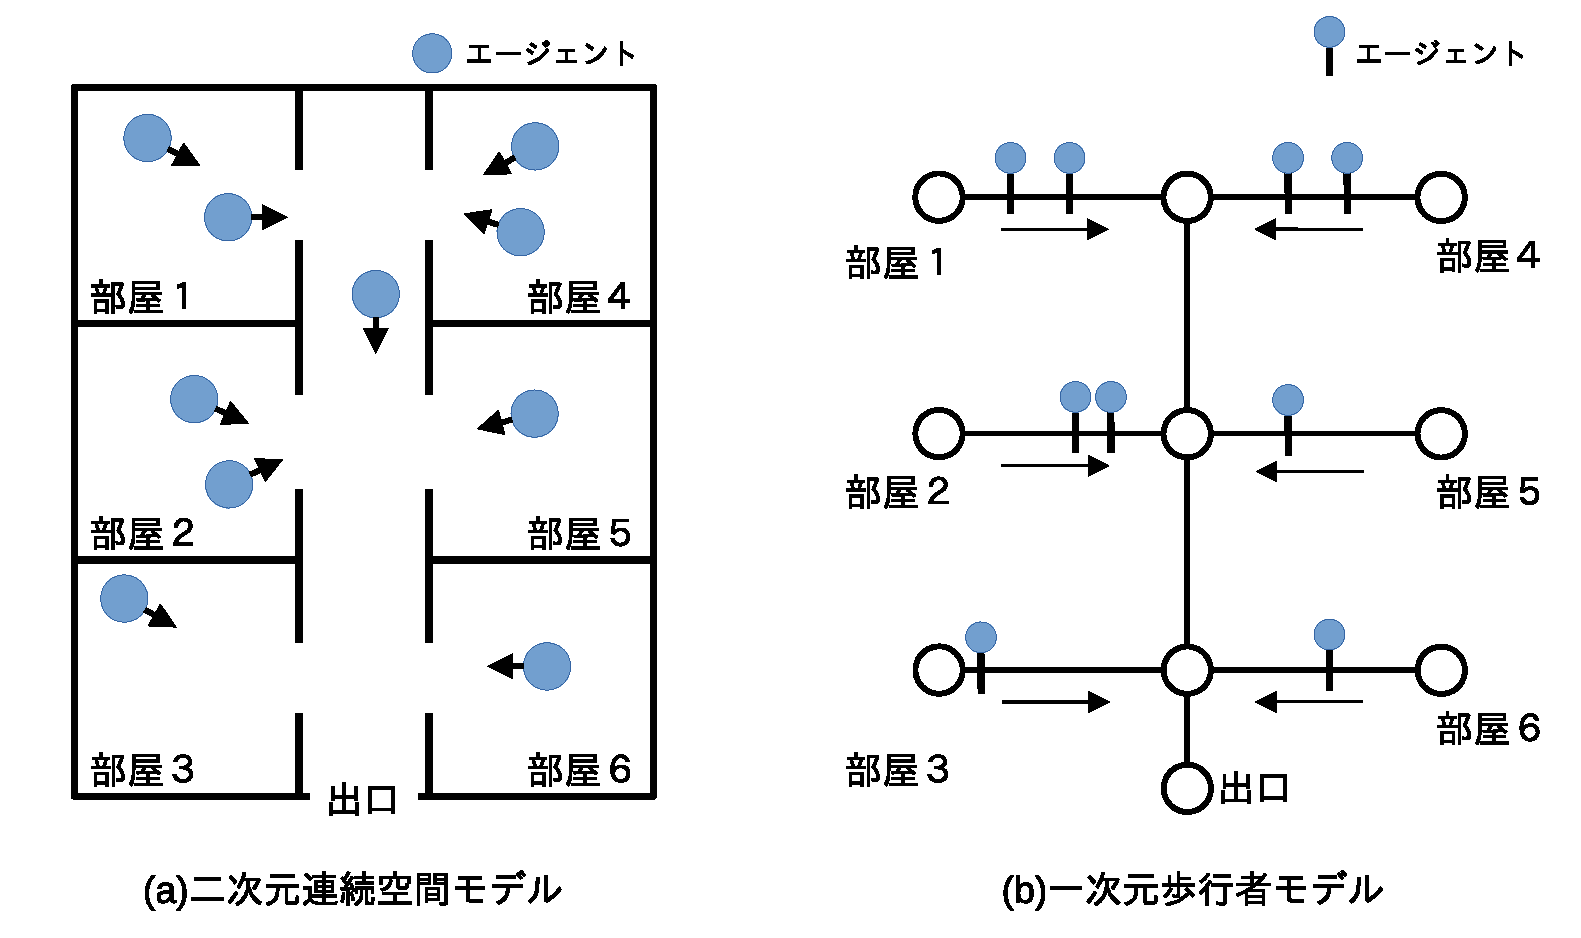
\includegraphics[width=11cm,clip]{figure/ichijigen_ex.eps}
  \caption{一次元モデルの例}
  \label{fig:atigenshou}
 \end{center}
\end{figure}

\begin{figure}[hbtp]
 \begin{center}
  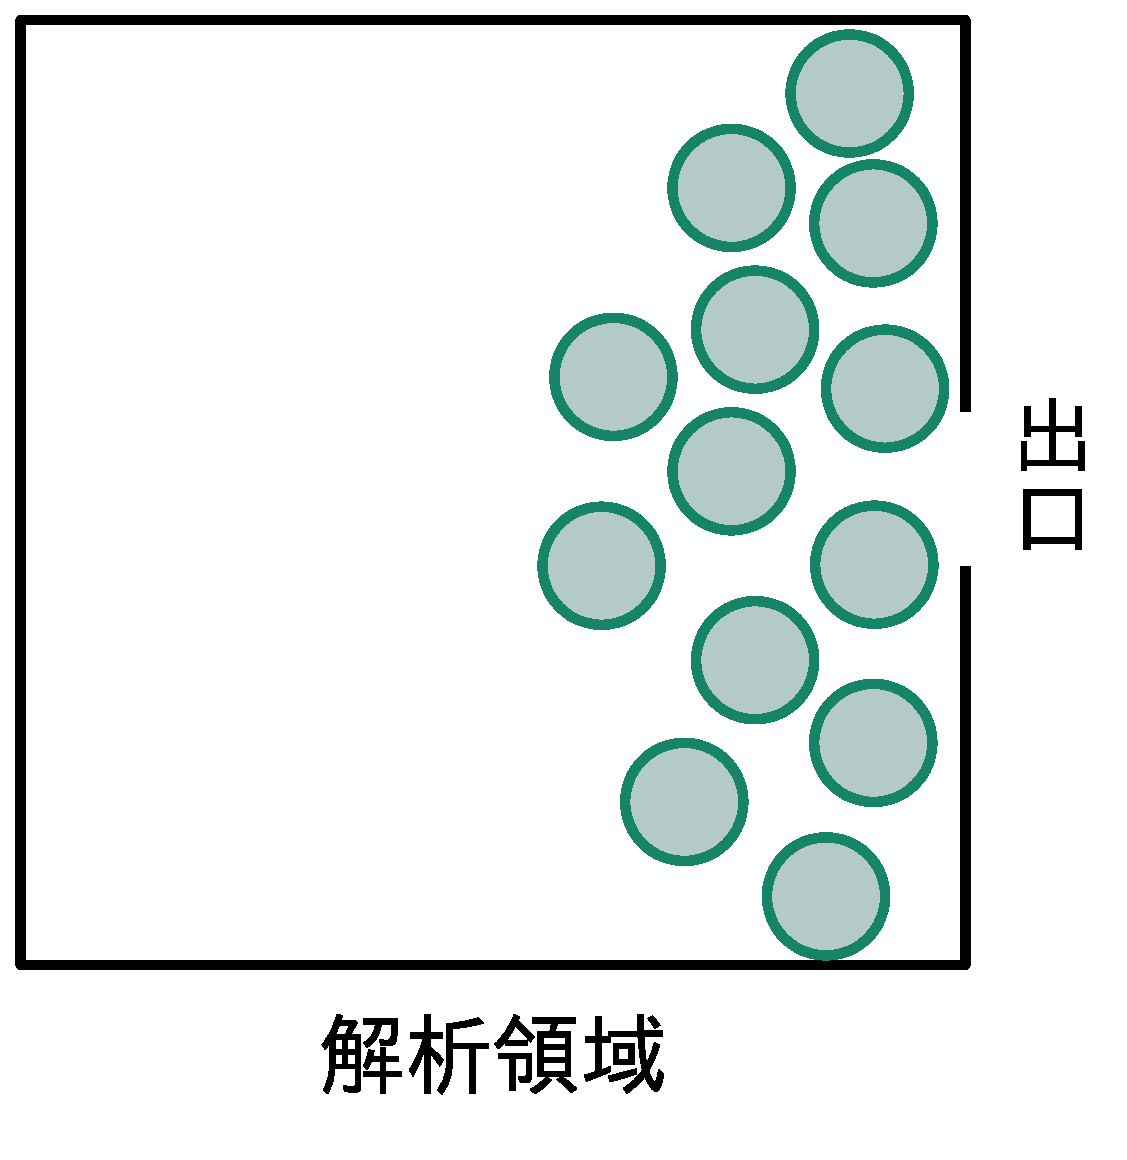
\includegraphics[width=5cm,clip]{figure/atigenshou.eps}
  \caption{アーチ現象の例}
  \label{fig:atigenshou}
 \end{center}
\end{figure}

\section{エージェント間の距離の計算回数削減}
SFMは,解析人数が増加するほど周囲のエージェントから受ける力の計算に
必要な周囲のエージェントが影響範囲内外かの判定の回数が増加する.
周囲のエージェントが影響範囲内外かの判定は,ルートなどを用いて
エージェント間距離$d_{ij}$を求める必要があるため,
特にエージェント間距離$d_{ij}$の計算に時間がかかる.
このため,SFMを用いた人流シミュレーションの解析時間を削減するためには,
エージェント間距離$d_{ij}$の計算回数を削減することが有効である.
エージェント間距離の計算回数削減手法にセル分割法や視野パラメータを用いた
削減手法がある.

\subsection{セル分割法}
セル分割法は,水や空気などの動きを解析できるMPS法\cite{mps}や銀河系などの圧縮性
流体に用いられるSPH法\cite{sph}などの粒子法によく用いられている.
粒子法は,近傍の粒子と相互作用する
力を計算し,粒子の行動を決定する.このため,セル分割法は,粒子法と同じように近傍の
エージェントとの相互作用力を計算するSFMに対しても用いられる.
本手法は,解析領域を格子上のセルに分割し,計算するエージェントの存在する
セルと近傍のセルに存在するエージェントに対して他のエージェントから受ける力の範囲であるか
判定し,範囲内であれば他のエージェントから受ける力を計算する手法である.
図\ref{fig:seru_ex1}にセル分割法を用いるSFMの例を示
す.図\ref{fig:seru_ex1}中の赤丸は他のエージェントから受ける力の計算をするエージ
ェント,黒丸は他のエージェント,四角は解析領域を格子状に分割したセルである.
この例では,エージェント4の行動を更新する際に青色のセル内に存在するエージェント
のみを参照するため,エージェント番号3,5,9の計算を削減できる.このとき,
視野を用いるSFMは,速度計算するエージェントの進行方向前方に存在するエージェント情報を
用いて計算するため,エージェントの進行方向後方のセルに存在するエージェント情報は不要になる,
このため,視野を用いるSFMでは,視野を考慮し,参照するセルを視野範囲に近づけることで,
計算回数を減らすことができる.

\begin{figure}[hbtp]
 \begin{center}
  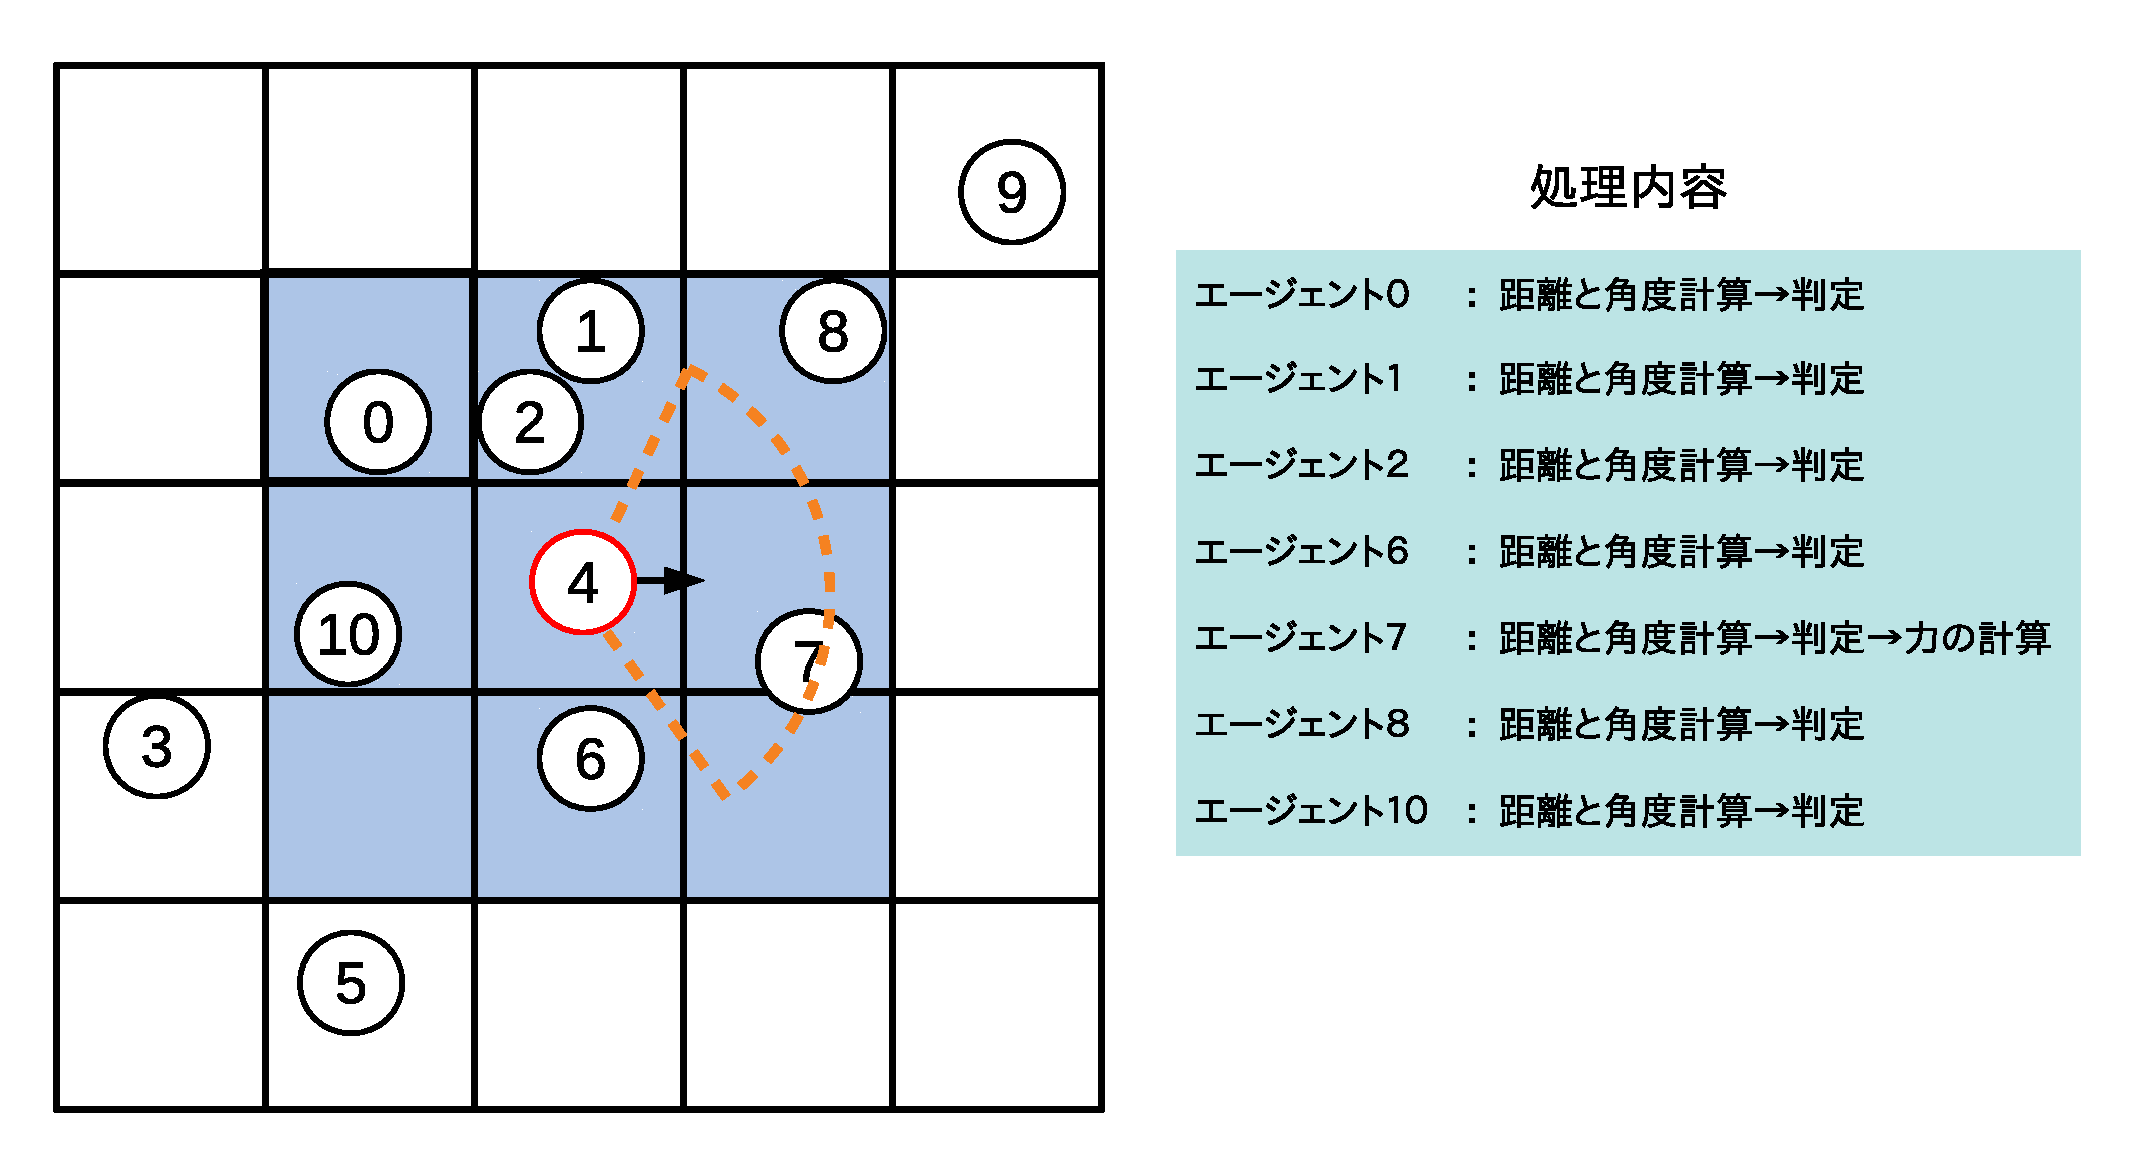
\includegraphics[width=11.5cm,clip]{figure/seru_ex1_r2.eps}
  \caption{セル分割法を用いた例}
  \label{fig:seru_ex1}
 \end{center}
\end{figure}


\subsection{視野パラメータを用いた削減手法}
視野パラメータを用いたSFMでは,


\section{単位時間あたりの計算回数}

\subsection{エージェントごとの並列性を用いた手法}

\begin{figure}[hp]
 \begin{center}
  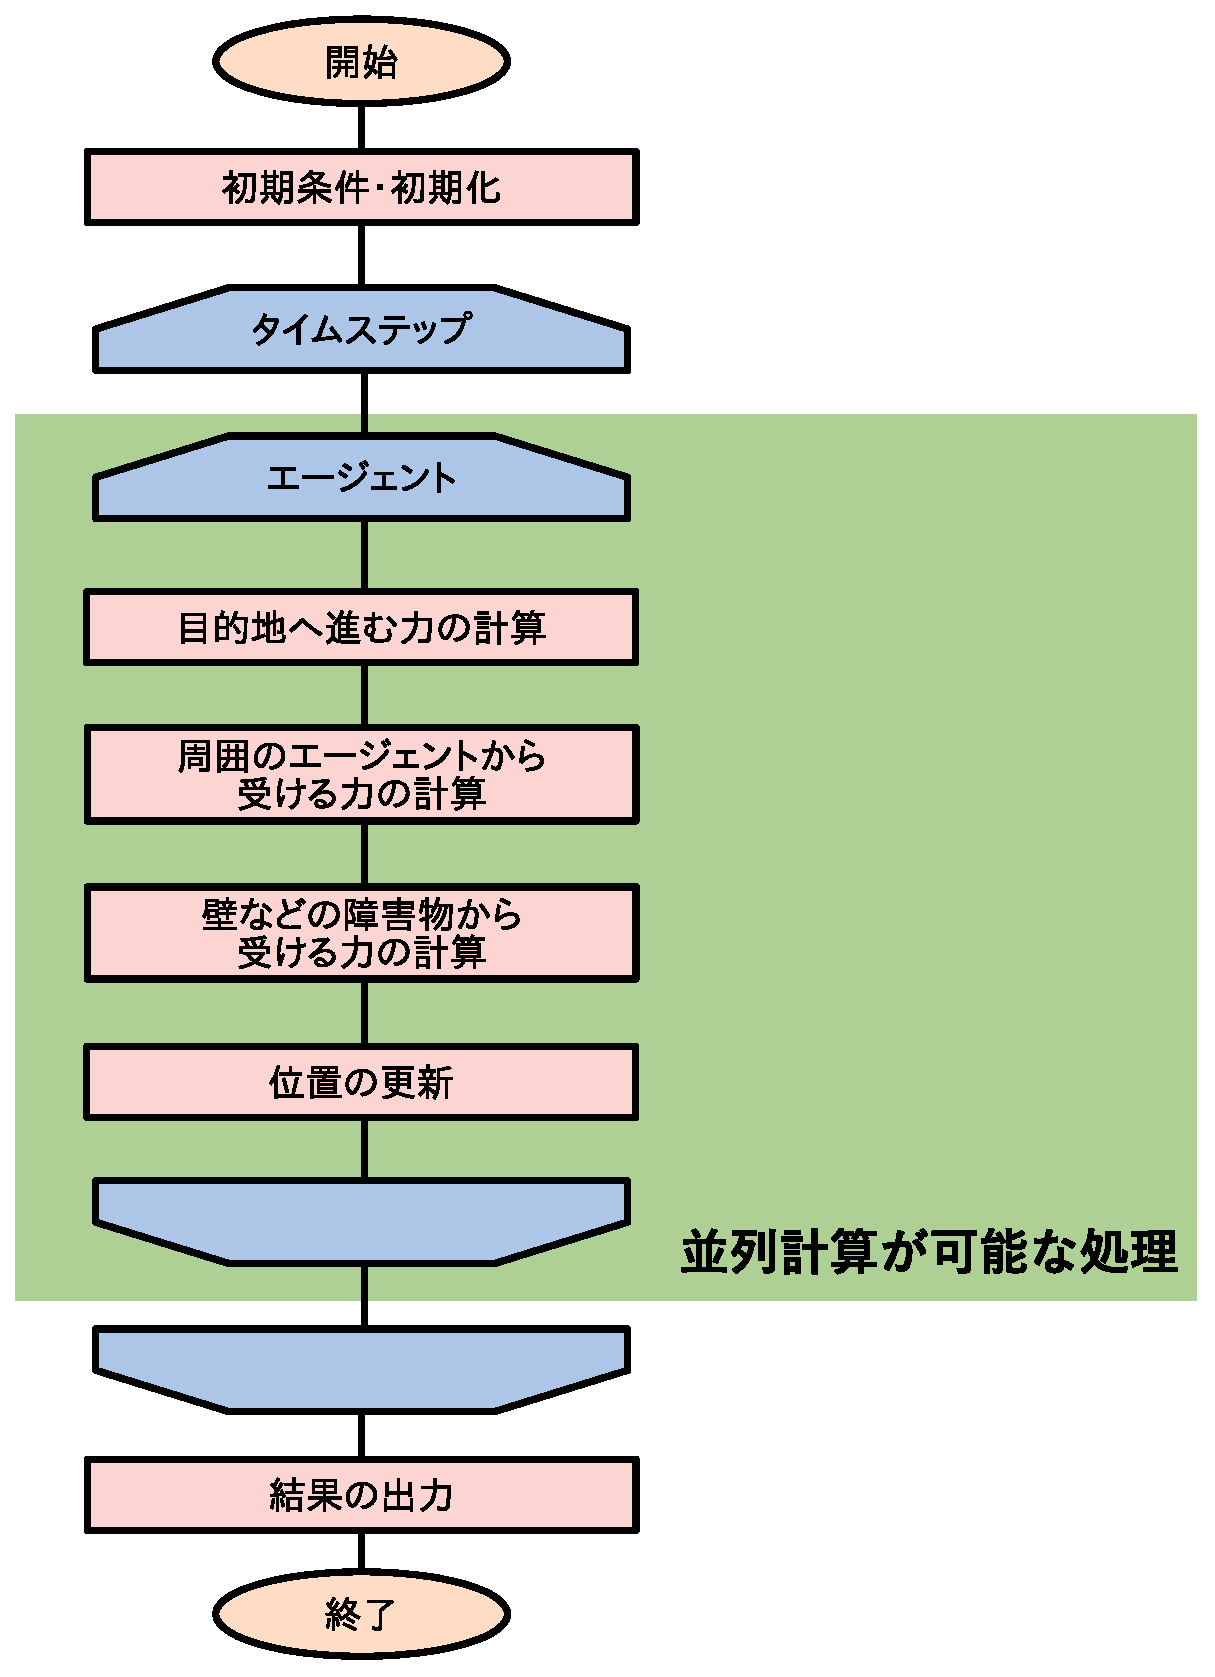
\includegraphics[width=10cm,clip]{figure/heiretuka_sfm.eps}
  \caption{SFMの並列化可能な処理}
  \label{fig:atigenshou}
 \end{center}
\end{figure}

\begin{figure}[hp]
 \begin{center}
  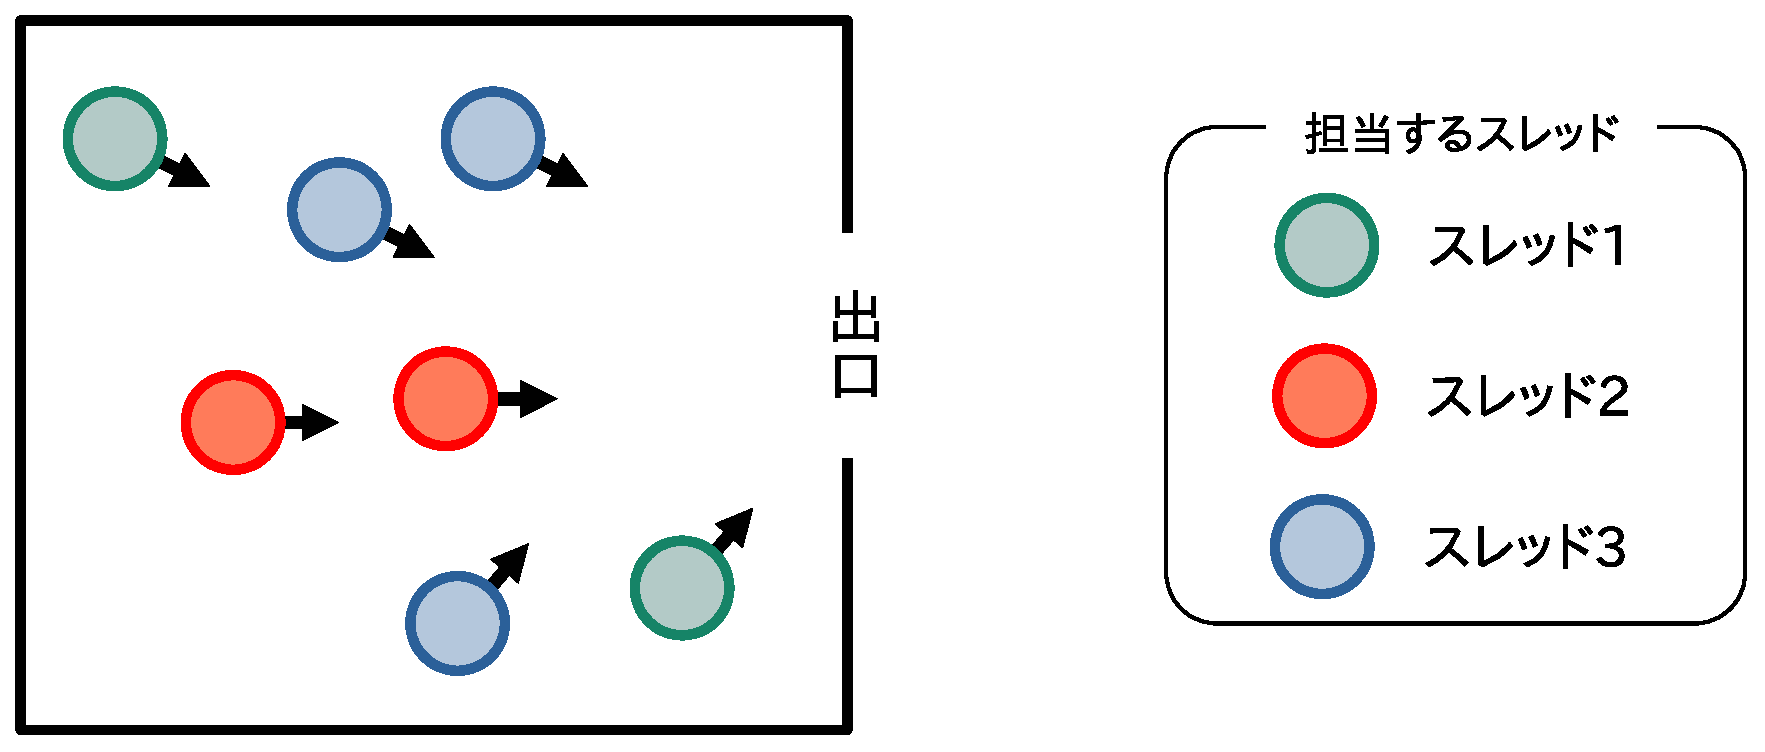
\includegraphics[width=10cm,clip]{figure/sureddo_heiretu.eps}
  \caption{3スレッドでの並列化の例}
  \label{fig:atigenshou}
 \end{center}
\end{figure}


\begin{figure}[hbtp]
 \begin{center}
  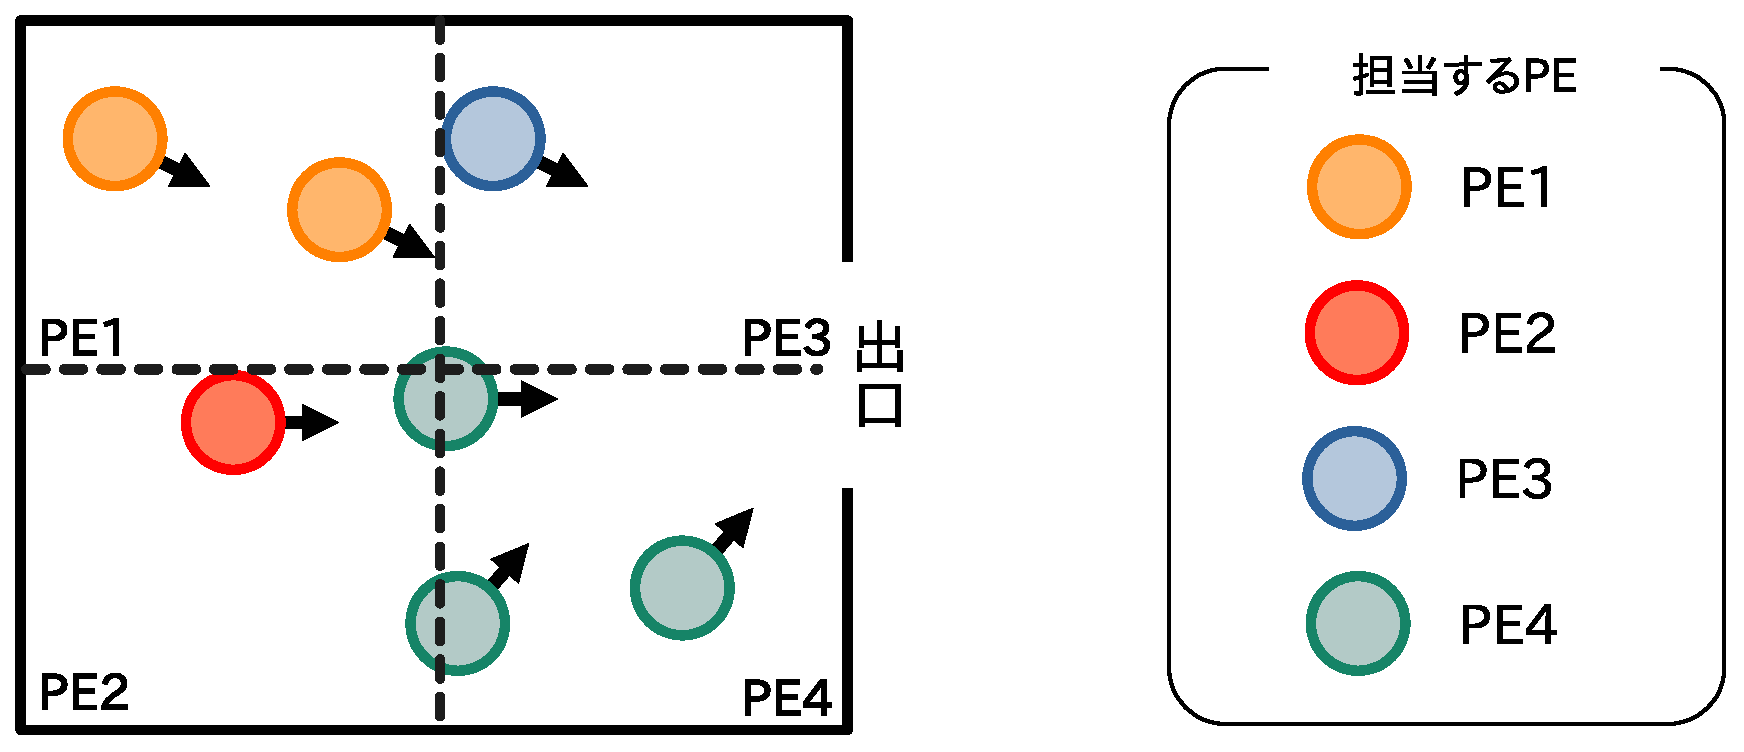
\includegraphics[width=10cm,clip]{figure/ryoiki_heiretu.eps}
  \caption{領域分割の例}
  \label{fig:atigenshou}
 \end{center}
\end{figure}


\clearpage

\subsection{解析領域ごとの並列性を用いた手法}

\section{経路選択時の判定回数削減}

\subsection{経路選択の単純化}

\subsection{経路選択手法の~~}




スタイルファイルの使い方について少し述べます.
普通に利用する分には,
拡張子が.texファイルのみを編集するだけで事が足りるように設計しました.
ただし,拡張子が.styファイルの書き換えは制限しません.自由に改変してください.


%----------------------------------------------------------
\section{abstract.tex}
%----------------------------------------------------------
abstract.texを書き換えると表紙およびアブストラクトを生成します.
abstract.tex内のコメントにしたがって書き換えを行ってください.
卒論にはアブストラクトが不要です.
修士のみアブストラクトを作成してください.

また,アブストラクトの設定はshuronABS.styに書いてあります.
表紙の設定はpenguin.styに書いてあります.
困ったときはこれらのファイルを変更してください.

%----------------------------------------------------------
\section{簡単コマンド}
%----------------------------------------------------------

penguin.styの294行目以降には, ショートカットコマンドを記述しました.
気が向いたら使ってやってください.
あくまでショートカットコマンドなので,
penguin.styのコマンドを使わなくても同じ機能を実現することができます.

\begin{itemize}
\item $\setminus$owata
\item $\setminus$ol\{ 数式 \}
\item $\setminus$fig\{ タイトル\}\{ ファイル名\}\{ 図の横幅[cm]\}
\item $\setminus$doublefig\{ タイトル1\}\{ ファイル名1\}\{ 図の横幅1[cm]\}\{ 図と図の間隔[cm]\}\{ title\_2\}\{ file\_name2\}\{ size\_2[cm]\}
\item $\setminus$figref\{ fig:ラベル\}
\item $\setminus$tabref\{ tb:ラベル\}
\end{itemize}


\figref{fig:ulysses16}に,$\setminus$figコマンドを用いて図を貼る例を示します.
\figref{fig:ulysses16}は,
$\setminus$fig\{適当な図を張ってみた\}\{ulysses16\}\{5\}で貼り付けています.
\figref{fig:ulysses16}では,図の横幅が5cmになるように大きさ指定をしています.


また,\figref{fig:test1}と\figref{fig:test2}は,
$\setminus$doublefigコマンドを用いて図を並べた例です.
これらの図は,$\setminus$doublefig\{横並び(左)\}\{test1\}\{2.5\}\{0.5\}\{横並び(右)\}\{test2\}\{2.5\}
で貼り付けています.
$\setminus$doublefigコマンドは,図のタイトル高さを自動調節する機能を持っていません.
このため,タイトルの高さは手動で調節してください.

\fig{適当な図を張ってみた}{ulysses16}{5}
\doublefig{横並び(左)}{test1}{2.5}{0.5}{横並び(右)}{test2}{2.5}

図を入れる時には,段落と段落の間に入れてください.
決して文の途中に図が入ることがあってはいけません.
もし,図を参照しているページと図のページが離れてしまった場合は,
段落の長さが適切でない可能性があります.
フォーマットを変えるのではなく,本文の構成を見直しましょう.


%----------------------------------------------------------
\section{参考文献}
\label{sec:bib}
%----------------------------------------------------------
参考文献を参照する文の例です\cite{1983_Ibaraki}.
参考文献の書き方には,bibファイルを使う方法と使わない方法の2通りがあります.
好きな方を選択し,makefileとmain.texを書き換えてください.

\subsection{bibファイルを使う場合}
main.texとmakefileの書き換えは必要ありません.
bibfile.bibに参考文献の記述例があります.
ciniiやIEEEなどでは文献のbibtex情報が用意されているので,
そのファイルをコピペして使えるのが強みです.
また,本方式を使うと,人力で参考文献情報をソートする必要が無いのでありがたいです.
ただし,参考文献が1つも参照されていないとエラーが生じる模様です\cite{test1}.

以下にFAQを載せておきます.
\begin{itemize}
        \item   {\bf bibファイルって何?bibtexって何?}\\
        使い方はgoogle先生に聞いてください.
        \item   {\bf 参考文献情報を書き換えてもコンパイル結果に反映されない}\\
        main.bblファイルを消去してから再コンパイルしてください.
        \item   {\bf 参考文献スタイルを変更したい}\\
        参考文献のフォーマットを決めるファイルは,sty/ipsjunsrt.bstです.
        本ファイルは,情報処理学会のスタイルファイルです.
        \item   {\bf 名字が1文字の人の表示がおかしい}\\
        情報処理学会フォーマットの仕様です.論文提出直前にbblファイルを直接編集してください.
        \item   {\bf bibファイルでエラーが出る}\\
        大抵の場合はカンマ忘れが原因です.次点で参照タグ名の重複かな?
\end{itemize}



\subsection{bibファイルを使わない場合}
自力でthebibliographyの中身を書くパターンです.
bibfile.texに記述例があります.
記述した通りに表示されるため,直感的には分かりやすいです.
ただし,人力での作業量が多くなるので,この方式を使う場合は頑張ってください.

本方式を用いる場合は,以下のファイルの書き換えが必要です.

\begin{itemize}
        \item {\bf main.tex\ }  61行目($\setminus$bibliography\{bibfile\})をコメントアウトし,
                                                62行目($\setminus$input\{bibfile\})のコメントアウトをはずしてください
        \item {\bf makefile\ }  $\#$記号でコメントアウトしてください
        \item {\bf bibfile.tex\ }       ここに参考文献を書いてください.
                                                参考文献は,本文中での参照順番に手動で並び替えが必要です.
\end{itemize}

%***** END ************************************************
